\begin{sidewaysfigure}[htbp]
\centering 
  \subfloat[\acs{mus} = 0.1, \acs{mur} = 0.4, $v_{inlet}$ = 100 m/s .]
  {
	  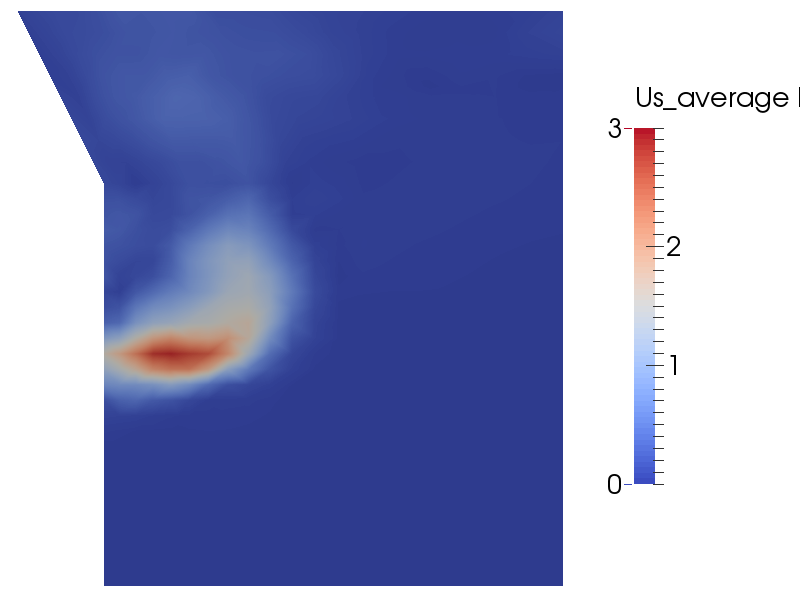
\includegraphics[width=.3\columnwidth]{images/231us_average_lf}
	  \label{fig:231us_average_lf}
  }
  \quad
    \subfloat[\acs{mus} = 0.5, \acs{mur} = 0.4, $v_{inlet}$ = 100 m/s .]
    {
	  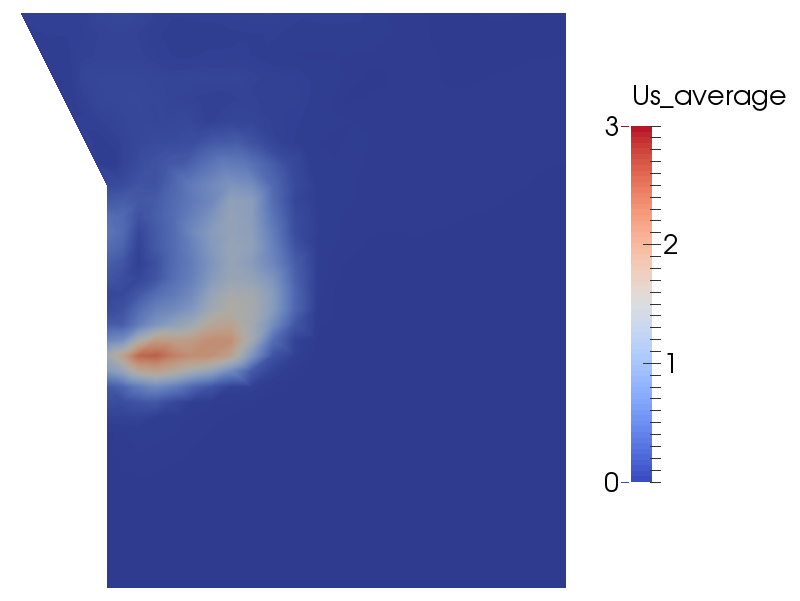
\includegraphics[width=.3\columnwidth]{images/248us_average_mf}
	  \label{fig:248us_average_mf}
  }
  \quad
    \subfloat[\acs{mus} = 0.9, \acs{mur} = 0.4, $v_{inlet}$ = 100 m/s .]
    {
	  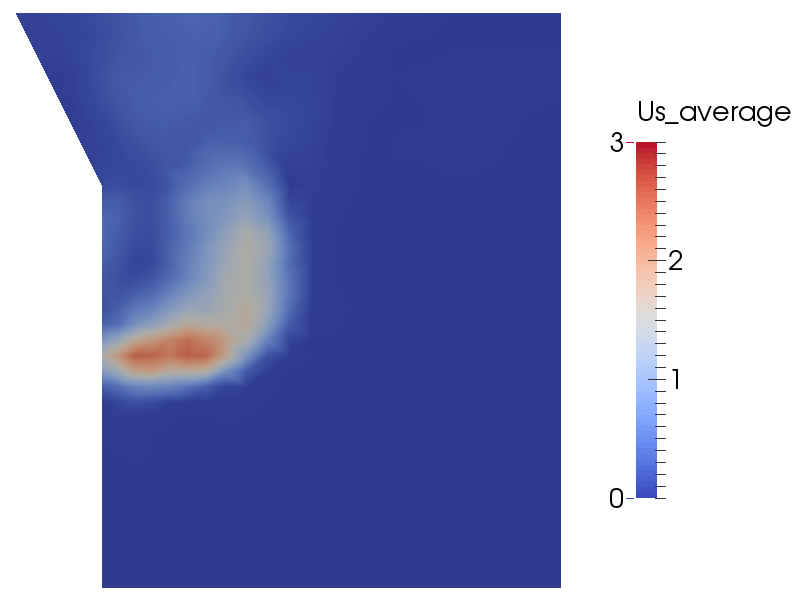
\includegraphics[width=.3\columnwidth]{images/230us_average_hf}
	  \label{fig:230us_average_hf}
  }
  \\
  \subfloat[\acs{mus} = 0.1, \acs{mur} = 0.4, $v_{inlet}$ = 200 m/s .]
  {
	  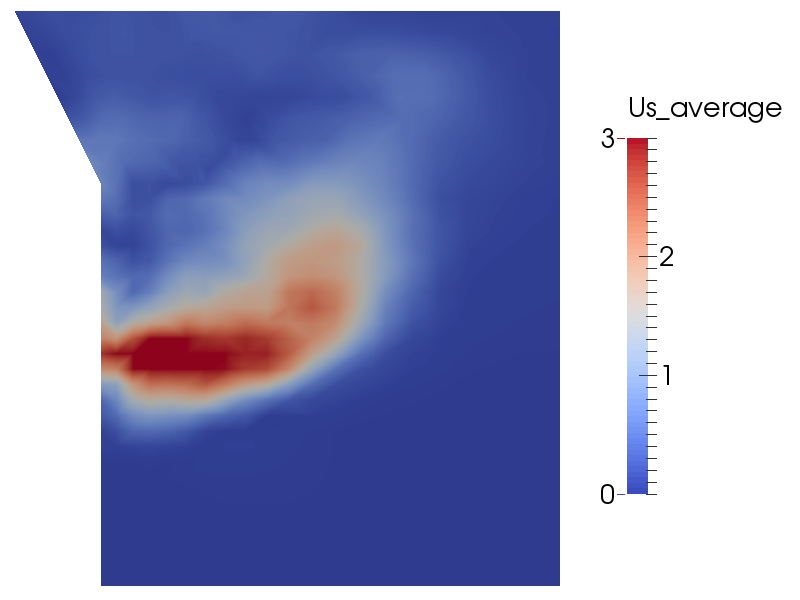
\includegraphics[width=.3\columnwidth]{images/247us_average_lfhv}
	  \label{fig:247us_average_lfhv}
  }
  \quad
    \subfloat[\acs{mus} = 0.9, \acs{mur} = 0.8, $v_{inlet}$ = 100 m/s .]
    {
	  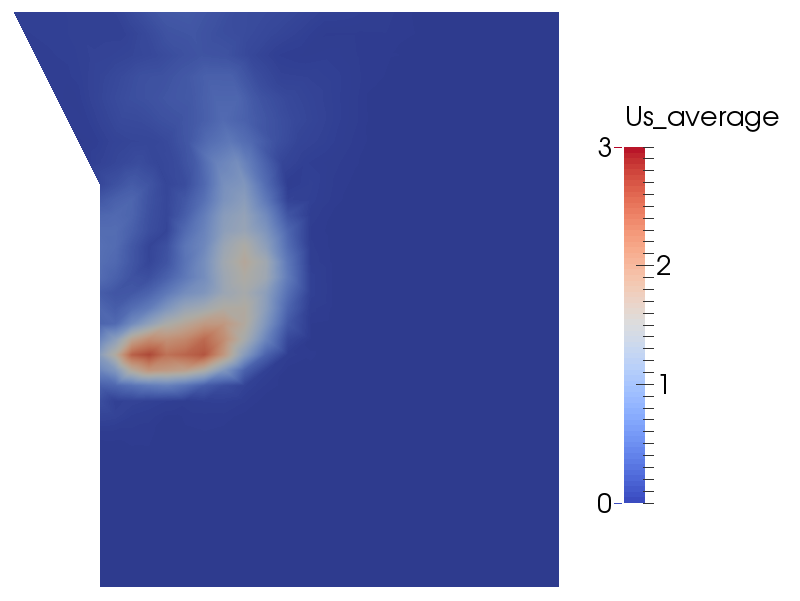
\includegraphics[width=.3\columnwidth]{images/246us_average_hfhr}
	  \label{fig:246us_average_hfhr}  }
  \\
  \caption{Average particle velocity with different sliding friction
  coefficient.}
  \label{fig:238racewayus}
\end{sidewaysfigure}